\section{Results}
If not stated differently the simulations use parameters as given in the table below:
\begin{table}[H]
    \centering
    \begin{tabular}{r|l}
        $N$ & $10^{5}$\\
        $D$ & $0,05$\\
        $R_s$ & $1$ \\
        $R_d$ & $10$ \\
        ${\rm d}t$ & $10^{-3}$
    \end{tabular}
    \caption{Default simulation parameters without potential barrier}
    \label{tab:Parameters_np}
\end{table}

\subsection{Ideal Sink without Potential Barrier}
The following figures show results of simulations using the model explained before. First we examine the dependence of the reaction rate on the diffusion constant. Therefore the simulation results are compared to the steady state analytic solution as given in \eqref{normalization}:
\begin{align}
    K &= 4 \pi R_s D \rho_o \\
    \rho_o &= N \left\{ \int_{R_s}^{R_d} \left( 1 - \frac{R_s}{r} \right) {\rm d} r \right\}^{-1}
    \label{Steady_state_rate}
\end{align}
\newpage
\subsubsection{Varying Diffusion Coefficient$D$}
\begin{figure}[H]
    \centering
    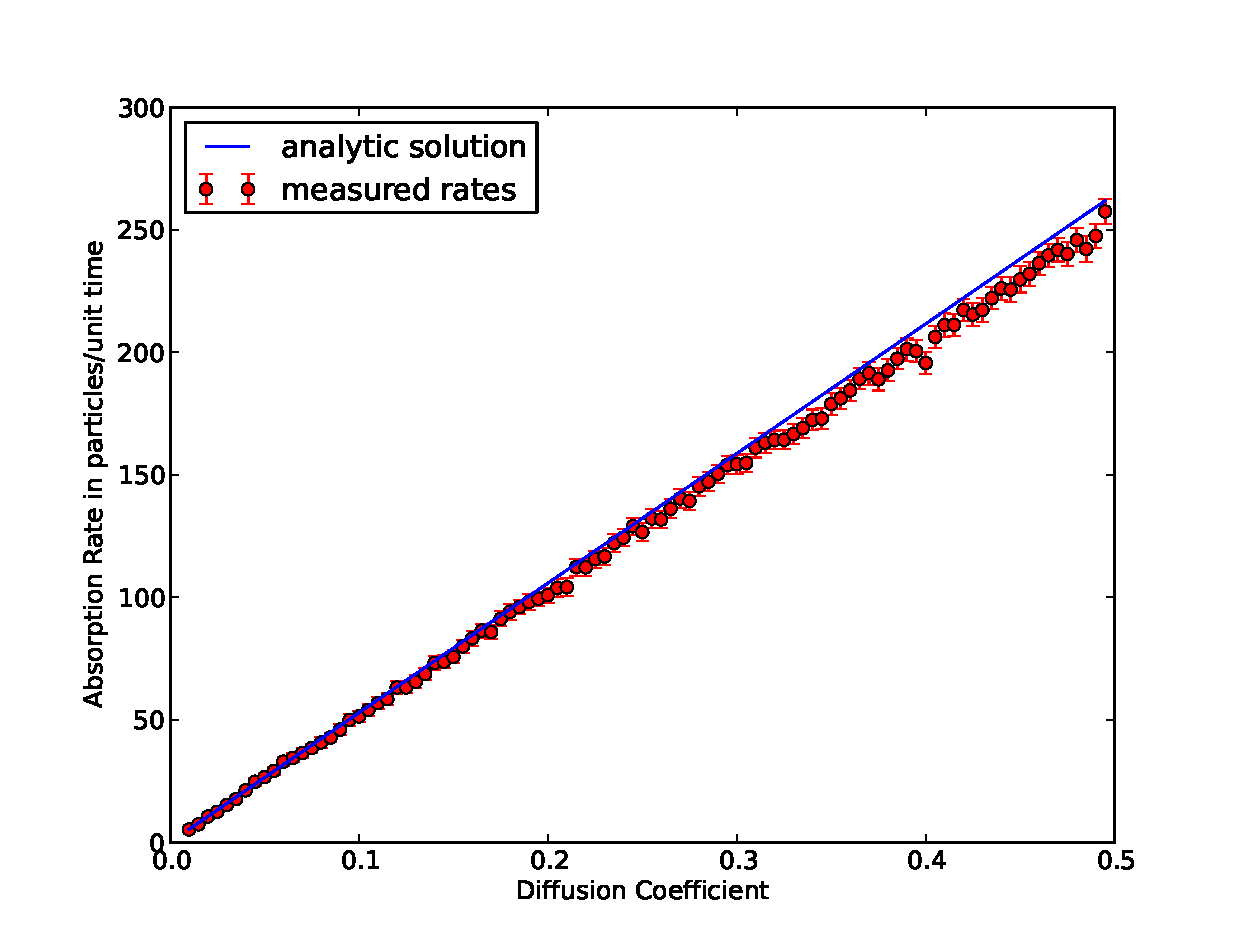
\includegraphics[width=.85 \textwidth, keepaspectratio]{plots/np/d/Kabs.eps}
    \caption{Reaction rates vs. Diffusion coefficient - Analytic solution and measured results}
    \label{fig:Kabs_D}
\end{figure}
\begin{wrapfigure}[17]{O}{.6 \textwidth}
    \centering
    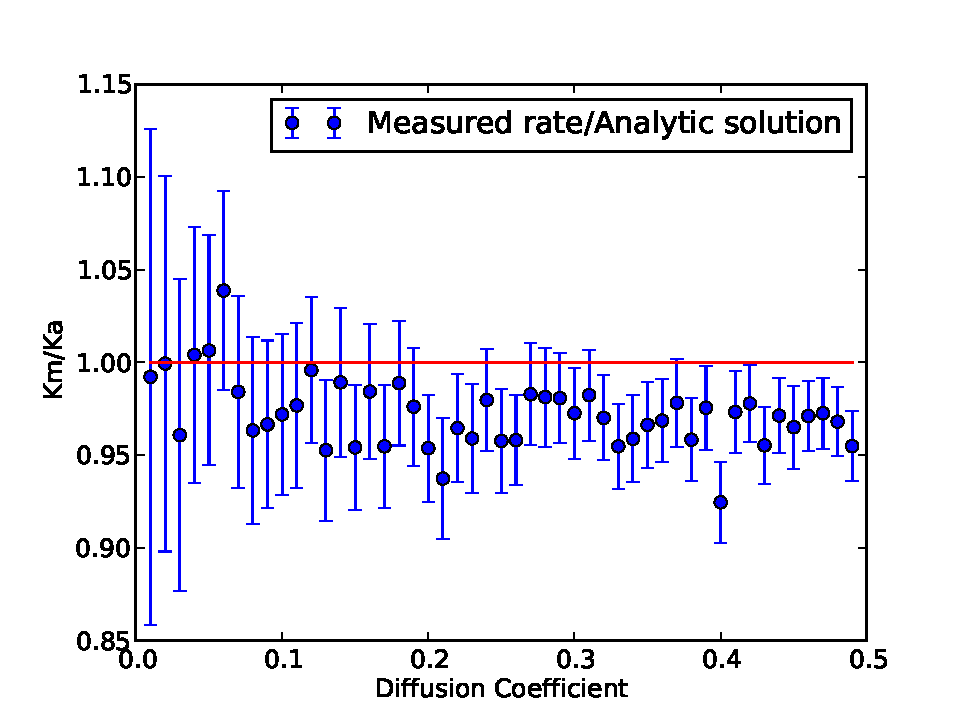
\includegraphics[width = .56 \textwidth, keepaspectratio]{plots/np/d/Krel.eps}
    \caption{Relative quantities for Reaction rates}
    \label{fig:Krel_d}
\end{wrapfigure}
The preceding figure shows the results for several simulation runs with different diffusion coefficient. It is obvious that the simulation results show the correct linear behaviour for the reaction rate but have a systematic error of about $5 - 10 \%$. To give a better impression of the relational dependence the following plot shows relative quantities for the results:
or $D > 0.1$ the figure shows a systematic error of about $5 \%$ in the results for the reaction rates. For $D<0.1$ the results are distributed around the analytic solution, mostly within the error bars, that are at  $2\sigma$. 
\newpage
\subsubsection{Varying Sink Radius $R_s$}
\begin{figure}[h]
    \centering
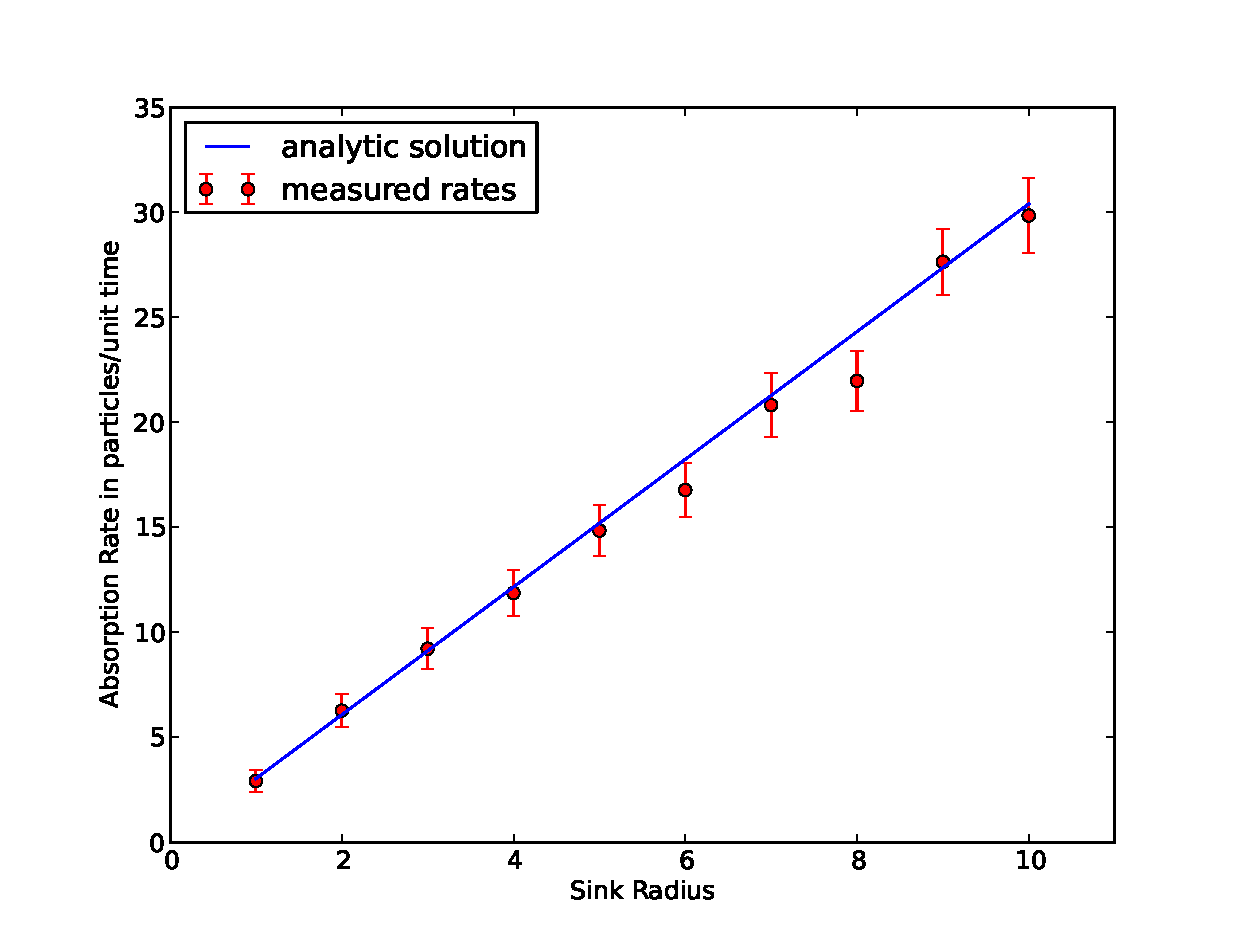
\includegraphics[width = .8 \textwidth]{plots/np/rs/KabsRs.eps}
    \caption{Reaction rate vs. Sink Radius}
    \label{fig:KabsRs}
\end{figure}
\begin{wrapfigure}[15]{O}{.6 \textwidth}
    \centering
    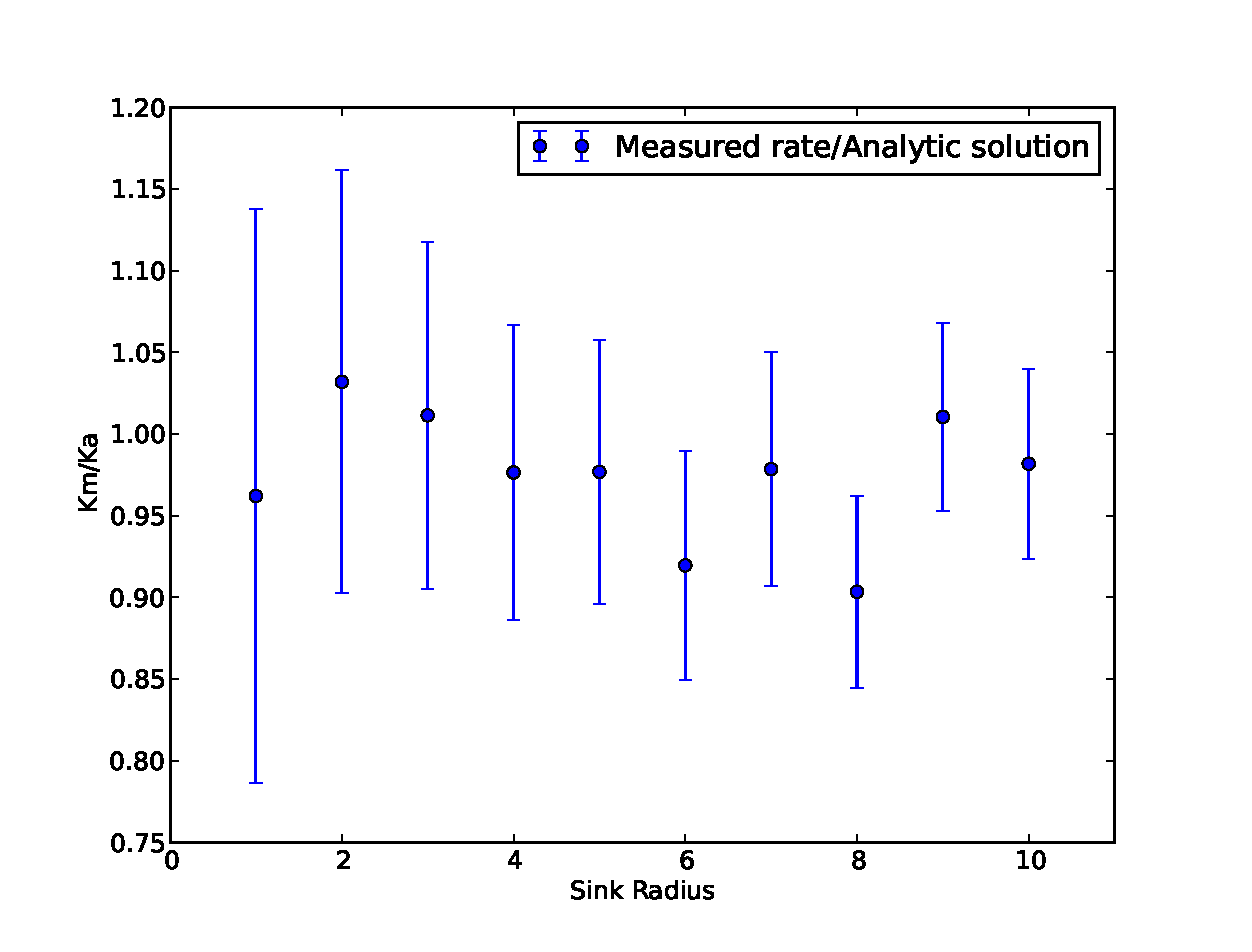
\includegraphics[width = .58 \textwidth]{plots/np/rs/KrelRs.eps}
    \caption{Normalized reaction rate vs. sink radius}
    \label{fig:KrelRs}
\end{wrapfigure}
This section gives results for different sink radius $R_s$ @ constant density $\rho_o$ to test the obvious linear relationship given in \eqref{Steady_state_rate}.
\
The results presented in the figure above do qualitatively support the linear relation between sink radius and reaction rate.
The adjacent strongly suggests, that the simulation also quantitatively maps on the analytic solution as the results are correct within the calculated errors at $2 \sigma$.
The following figures present the obtained density profiles from the simulation.
\begin{figure}[H]
    \centering
    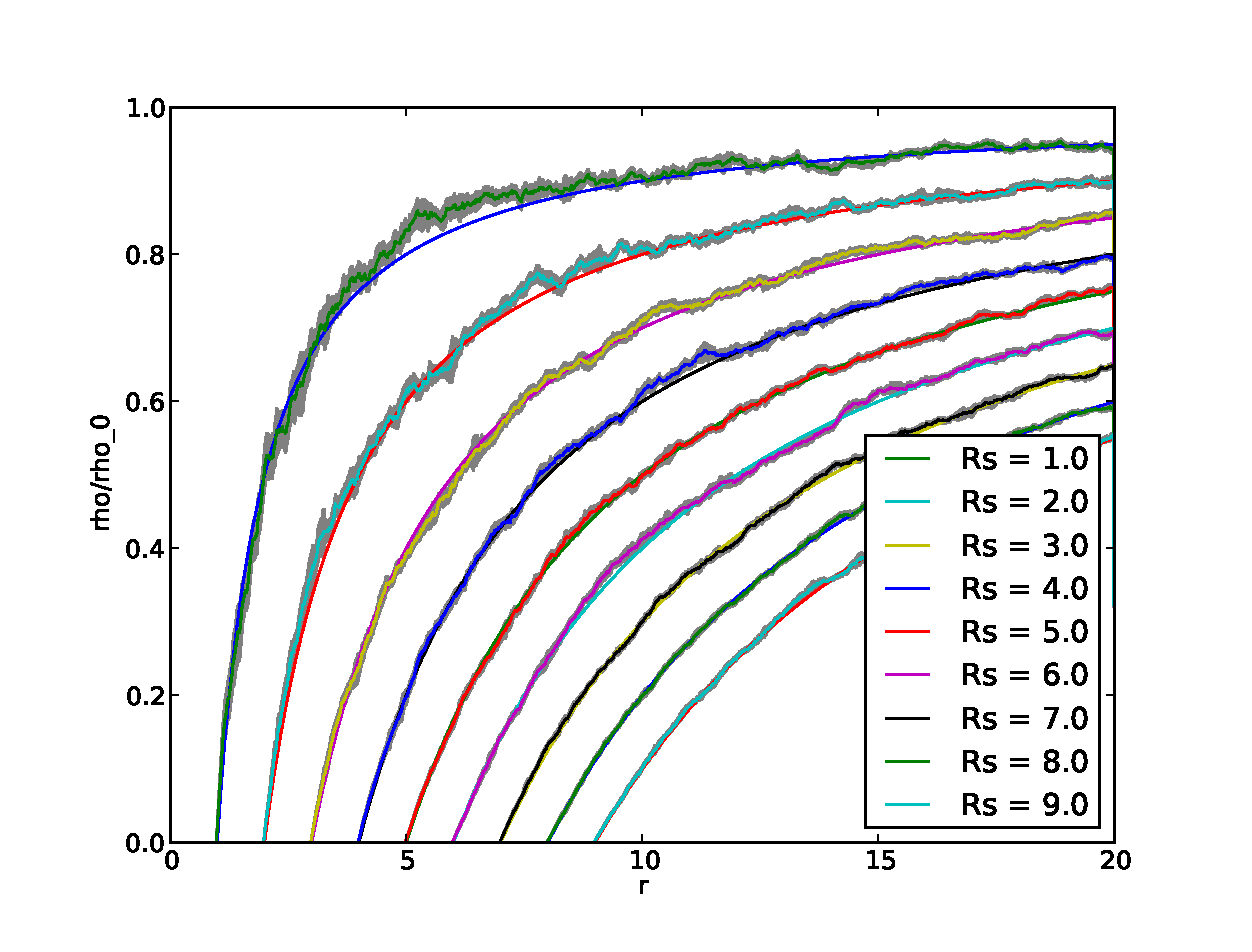
\includegraphics[width = .8 \textwidth]{plots/np/rs/rho_over_rho0.eps} 
    \caption{Normalized density profiles for different sink radius}
    \label{fig:ror0Rs}
\end{figure}
\begin{figure}[H]
    \centering
    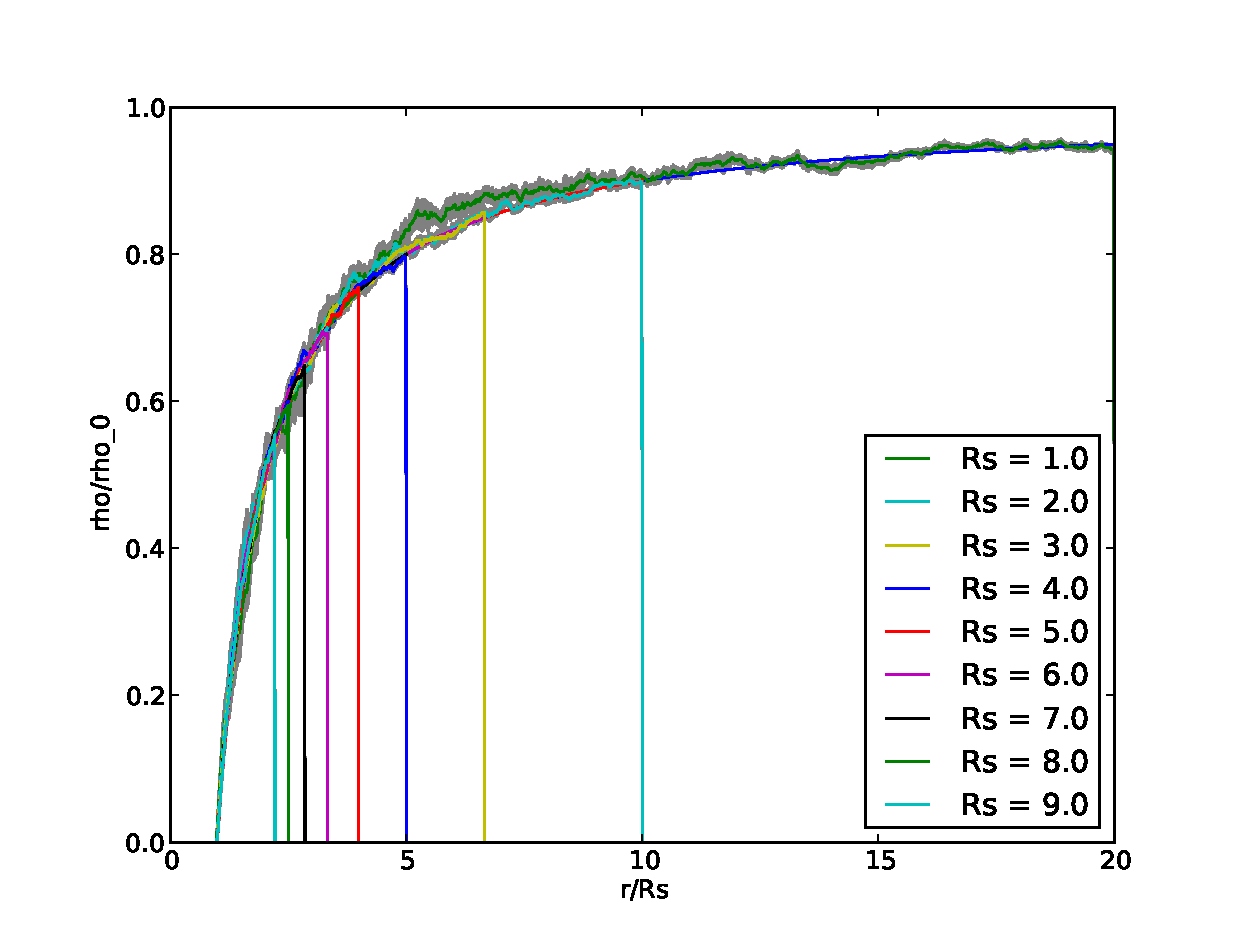
\includegraphics[width = .8 \textwidth]{plots/np/rs/rho_over_rho_0_rescaled.eps} 
    \caption{Normalized density profiles for different sink radius with rescaled radial coordinate}
    \label{fig:ror0Rs_rescaled}
\end{figure}
\newpage
\subsubsection{Finite size analysis - Varying Domain Radius $R_d$}
\begin{figure}[H]
    \centering
    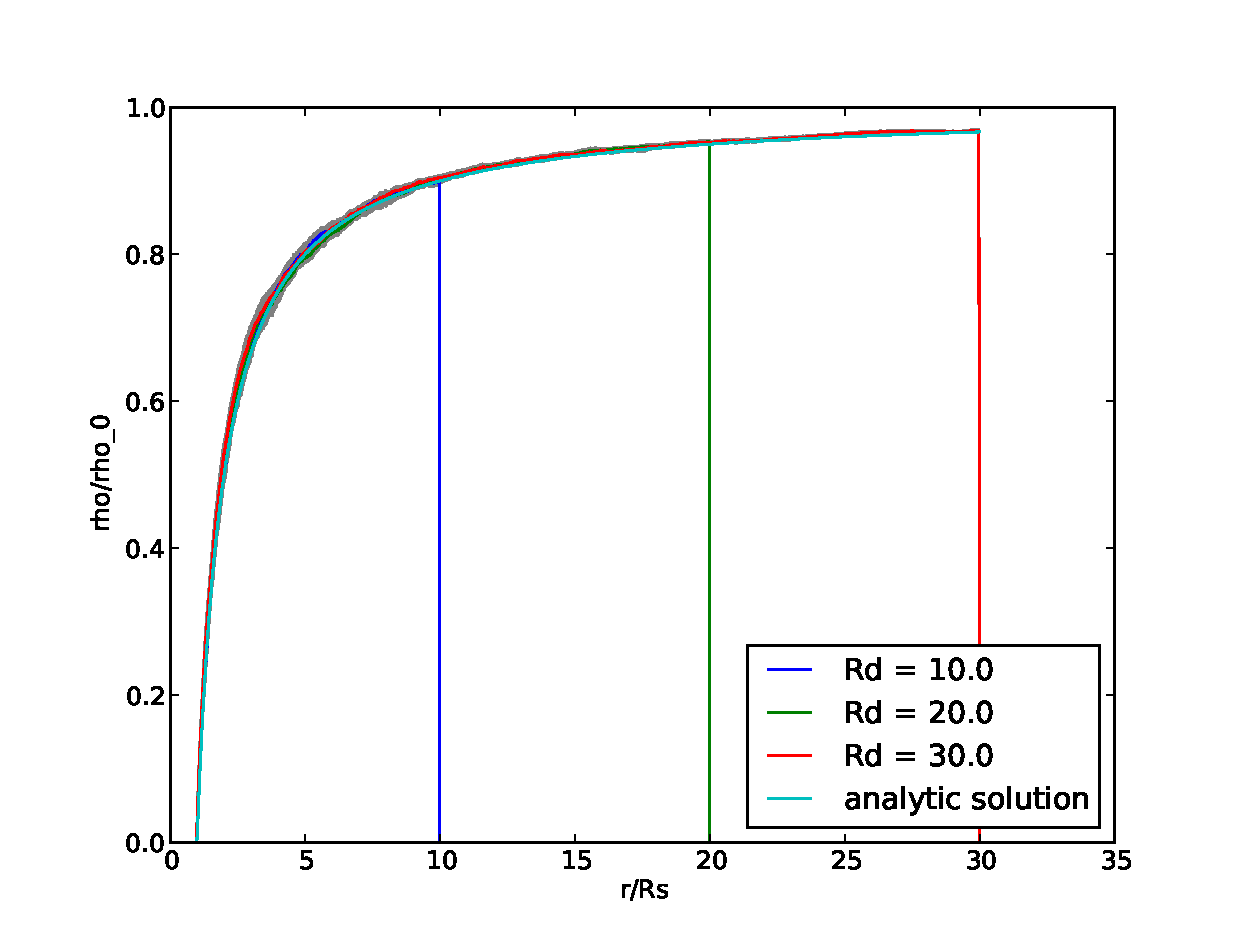
\includegraphics[width = .8 \textwidth]{plots/np/rd/rho_over_rho0.eps}
    \caption{Density profiles for different domain Radius $R_d$}
    \label{fig:ror0Rd}
\end{figure}
\begin{wrapfigure}[17]{O}{.6 \textwidth}
    \centering
    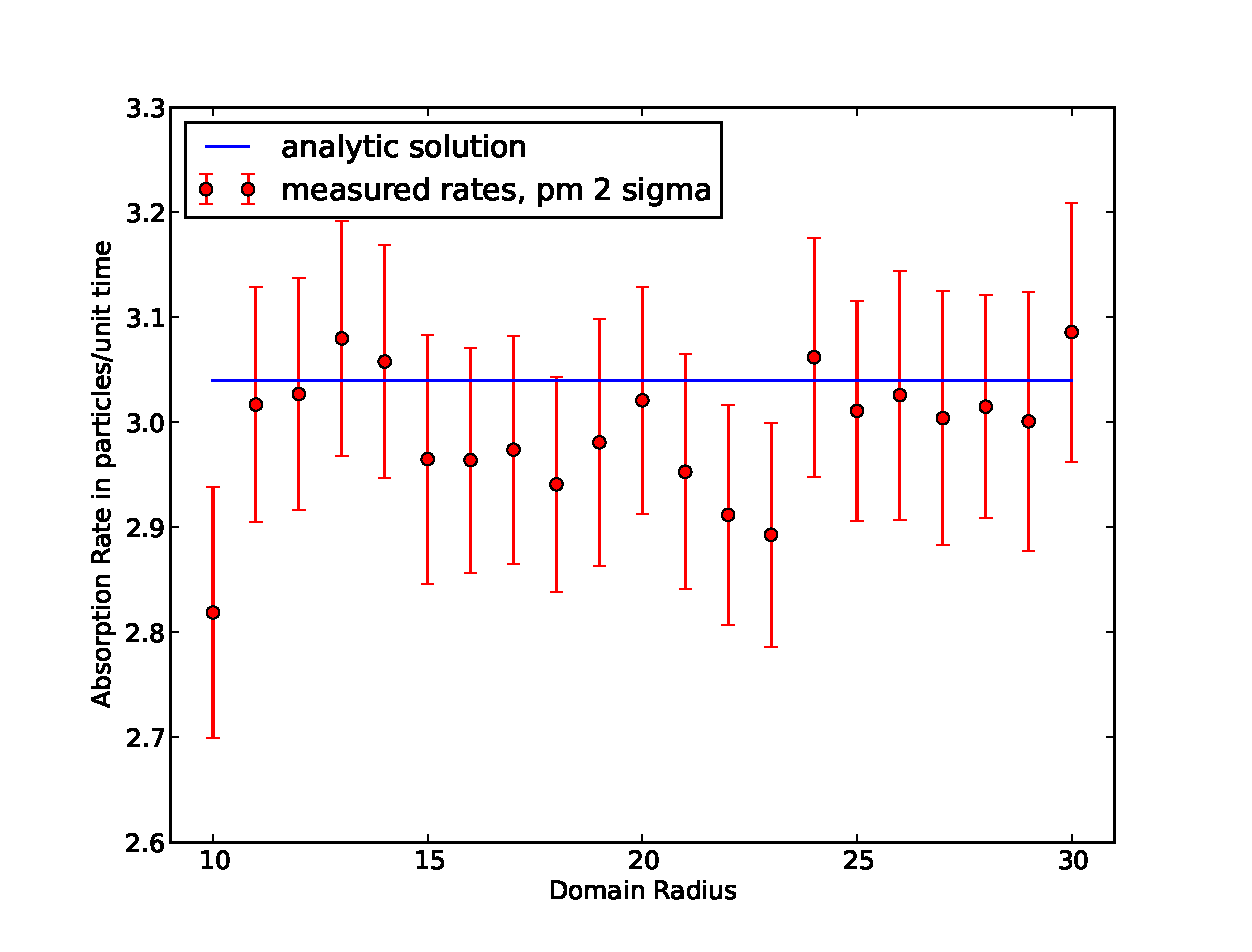
\includegraphics[width = .56 \textwidth]{plots/np/rd/KabsRd.eps}
    \caption{reaction rate vs. domain radius}
    \label{fig:KrelRd}
\end{wrapfigure}
This section shows plots for different domain radius $R_d$ @ constant density $\rho_o$.
This will point out finite size effects in the simulation (if they exist). To account for the larger volume the number of particles is adjusted to keep the solution for density profile and rate constants unchanged.
The plot above shows, that the variation of the domain radius does not qualitatively change the simulated density profile. \\
The results for the rate constants does not show any qualitative changes for varying domain radius. \\
These results suggest, that for the given boundary conditions and for ideal particles without external forces there are no finite size effects in this simulation.
\subsection{Subsumption}
The different results from simulation presented in the previous section show that:
\begin{itemize}
    \item The density profiles from the BD simulation fit the analytical solution,
    \item the obtained rate constants are as expected within the calculated errors
    \item   the diffusion constant and  or time step has to be small enough for the particle 
            trajectories to resolve the boundary conditions properly,
    \item finite size effects can be neglected.
\end{itemize}
\subsection{Ideal Sink with Boxcar Potential Barrier}
The following section contains simulation results for a potential barrier as derived in \eqref{Boxcar_solution}. If not stated differently, the following parameters are used:
\begin{table}[H]
    \centering
    \begin{tabular}{r|l}
        $N$ & $10^{4}$\\
        $D$ & $0,05$\\
        $R_s$ & $1$ \\
        $R_d$ & $10$ \\
        $U_0$ & $2$ \\
        $U_a$ & $2$ \\
        $U_b$ & $2$ \\
        $U_n$ & $50$ \\
        ${\rm d}t$ & $10^{-4}$
    \end{tabular}
    \caption{Default simulation parameters for simulation with boxcar potential}
    \label{tab:Parameters_cp}
\end{table}

\subsubsection{Varying Distance from Sink to Barrier ($U_a$)}
\begin{figure}[H]
\centering
\begin{minipage}{.5 \textwidth}
    \centering
    \includegraphics[width=.95 \textwidth, keepaspectratio]{plots/cp/ua/Ua1.eps}
\end{minipage}\begin{minipage}{.5 \textwidth}
    \includegraphics[width=.95 \textwidth, keepaspectratio]{plots/cp/ua/Ua3.eps}
\end{minipage}
\begin{minipage}{.5 \textwidth}
    \includegraphics[width=.95 \textwidth, keepaspectratio]{plots/cp/ua/Ua5.eps}
\end{minipage}\begin{minipage}{.5 \textwidth}
    \includegraphics[width=.95 \textwidth, keepaspectratio]{plots/cp/ua/Ua5.eps}
\end{minipage}
 
    \caption{Density Profile for varying $U_a$}
    \label{fig:RhoUaCp}
\end{figure}

The simulation results obviously fit the analytic solution. Same holds for the calculated reaction rates as presented in the following Plot:
\begin{figure}[H]
\centering
\begin{minipage}{.5 \textwidth}
    \centering
    \includegraphics[width=.95 \textwidth, keepaspectratio]{plots/cp/ua/Kabs.eps}
\end{minipage}\begin{minipage}{.5 \textwidth}
    \includegraphics[width=.95 \textwidth, keepaspectratio]{plots/cp/ua/Krel.eps}
\end{minipage}
\caption{Absolute and relative Absorption rate for varying $U_a$}
\label{fig:KUaCp}
\end{figure}

\subsubsection{Varying Barrier Height ($U_0$)}
\begin{figure}[H]
\centering
\begin{minipage}{.5 \textwidth}
    \centering
    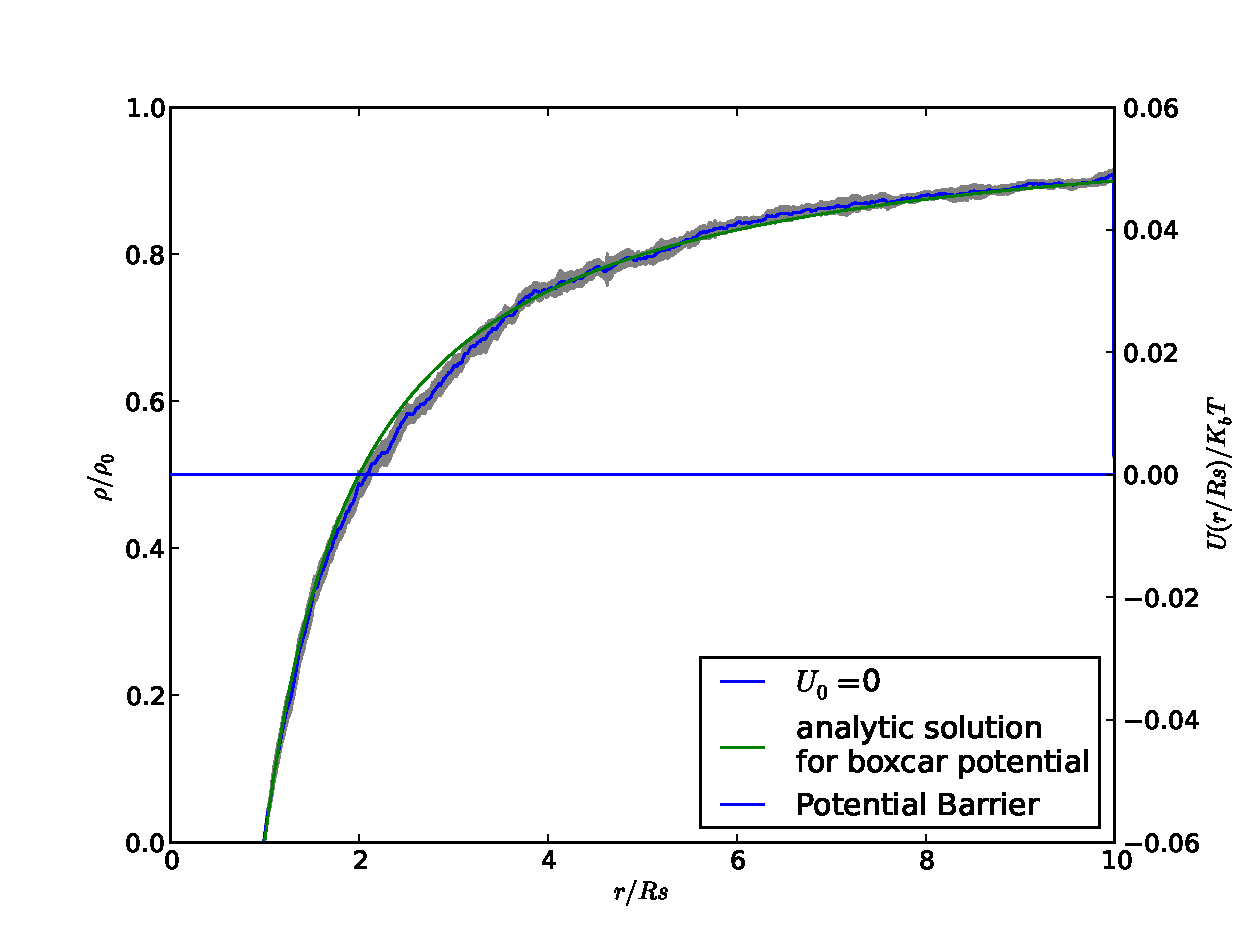
\includegraphics[width=.95 \textwidth, keepaspectratio]{plots/cp/uo/Un0.eps}
\end{minipage}\begin{minipage}{.5 \textwidth}
    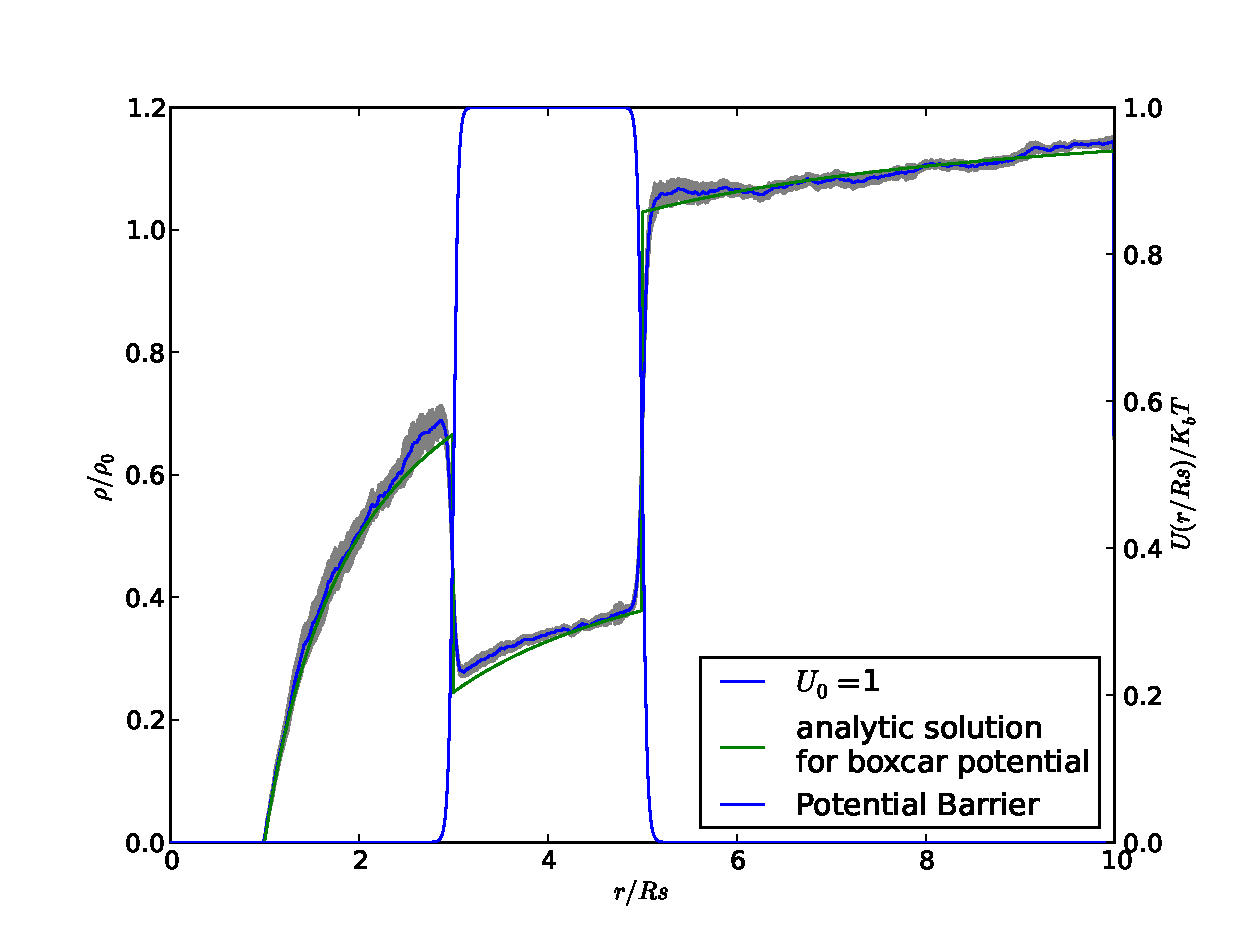
\includegraphics[width=.95 \textwidth, keepaspectratio]{plots/cp/uo/Un1.eps}
\end{minipage}
\begin{minipage}{.5 \textwidth}
    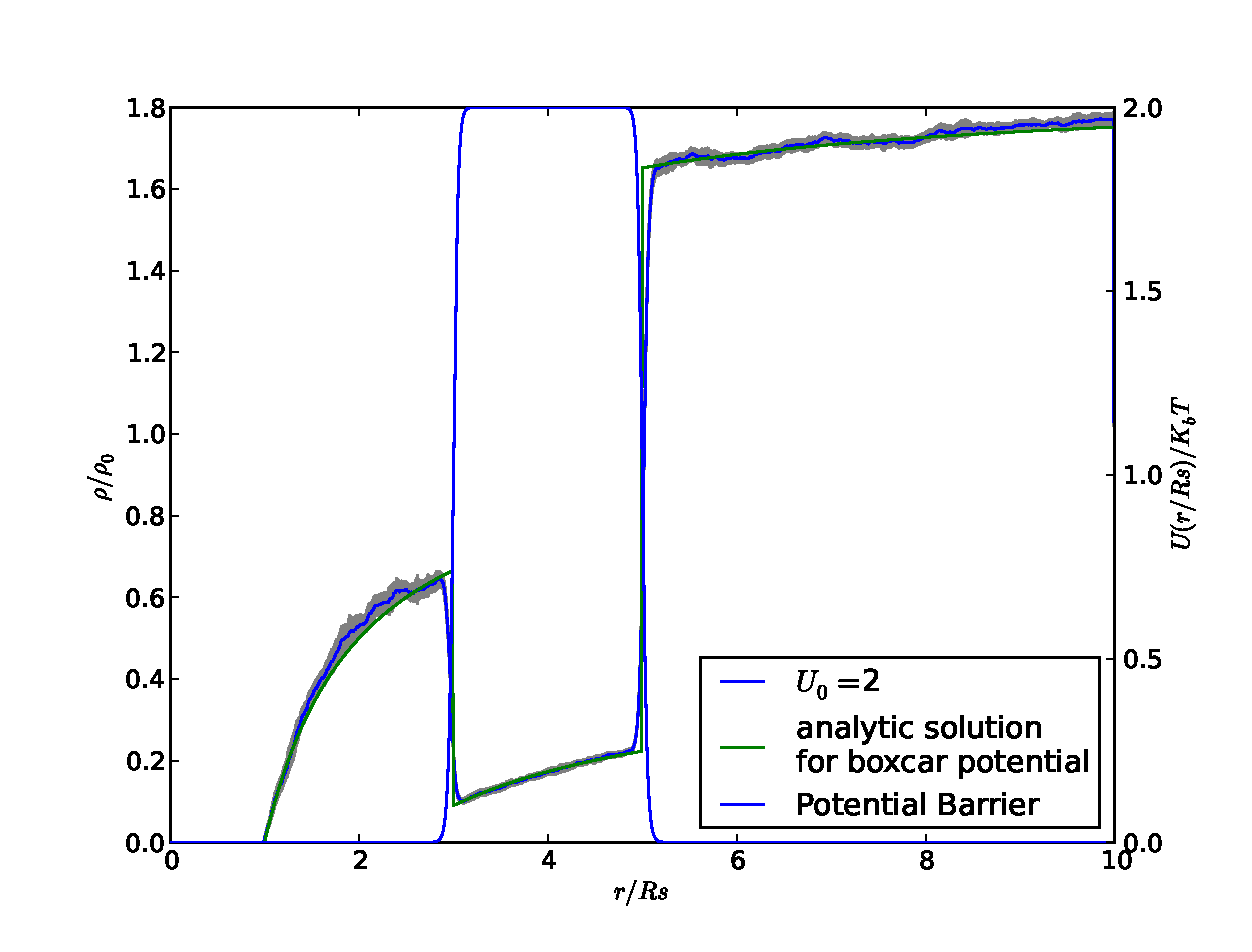
\includegraphics[width=.95 \textwidth, keepaspectratio]{plots/cp/uo/Un2.eps}
\end{minipage}\begin{minipage}{.5 \textwidth}
    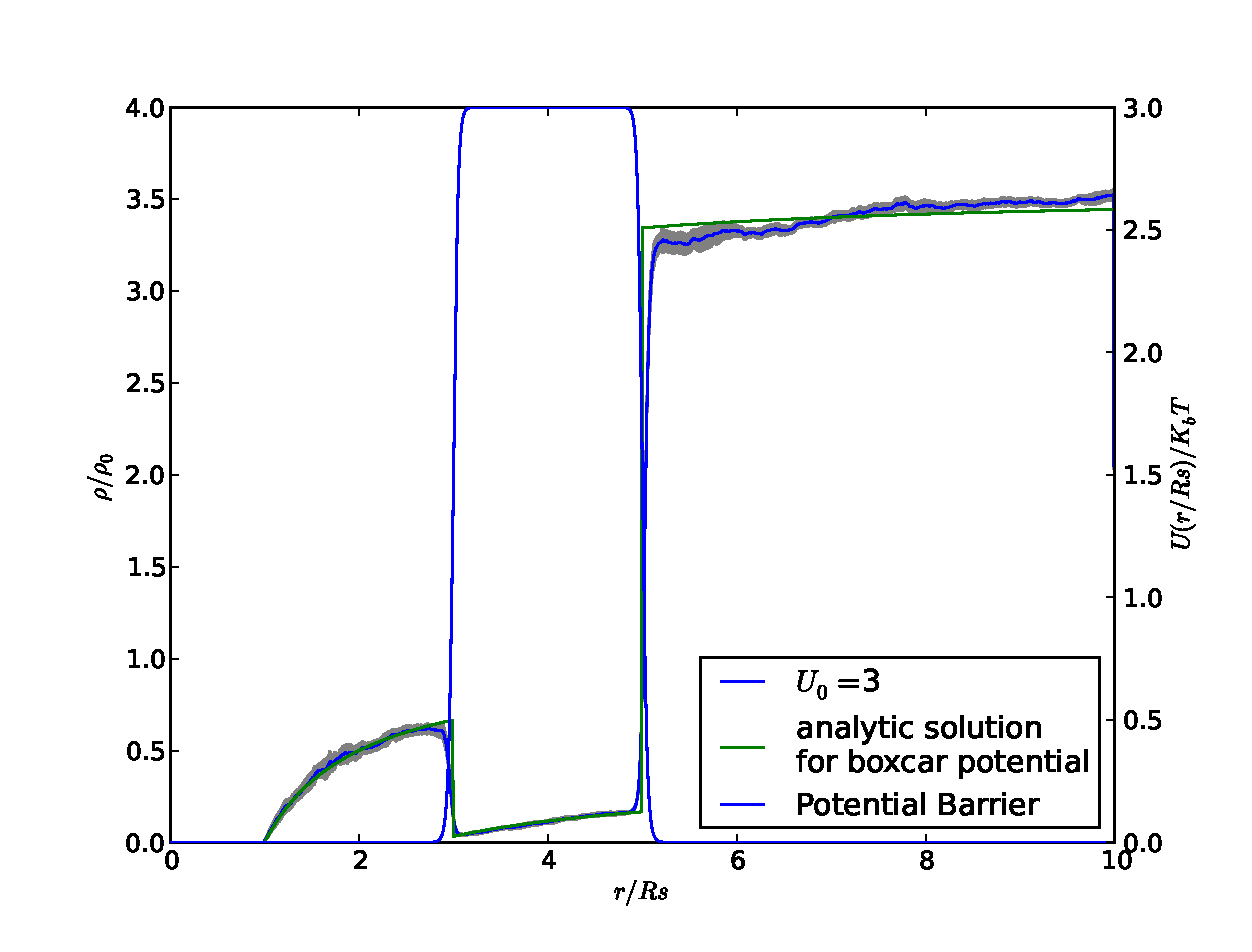
\includegraphics[width=.95 \textwidth, keepaspectratio]{plots/cp/uo/Un3.eps}
\end{minipage}
 
    \caption{Density Profile for varying $U_0$}
    \label{fig:RhoU0Cp}
\end{figure}

The simulation results obviously fit the analytic solution. Same holds for the calculated reaction rates as presented in the following Plot:
\begin{figure}[H]
\centering
\begin{minipage}{.5 \textwidth}
    \centering
    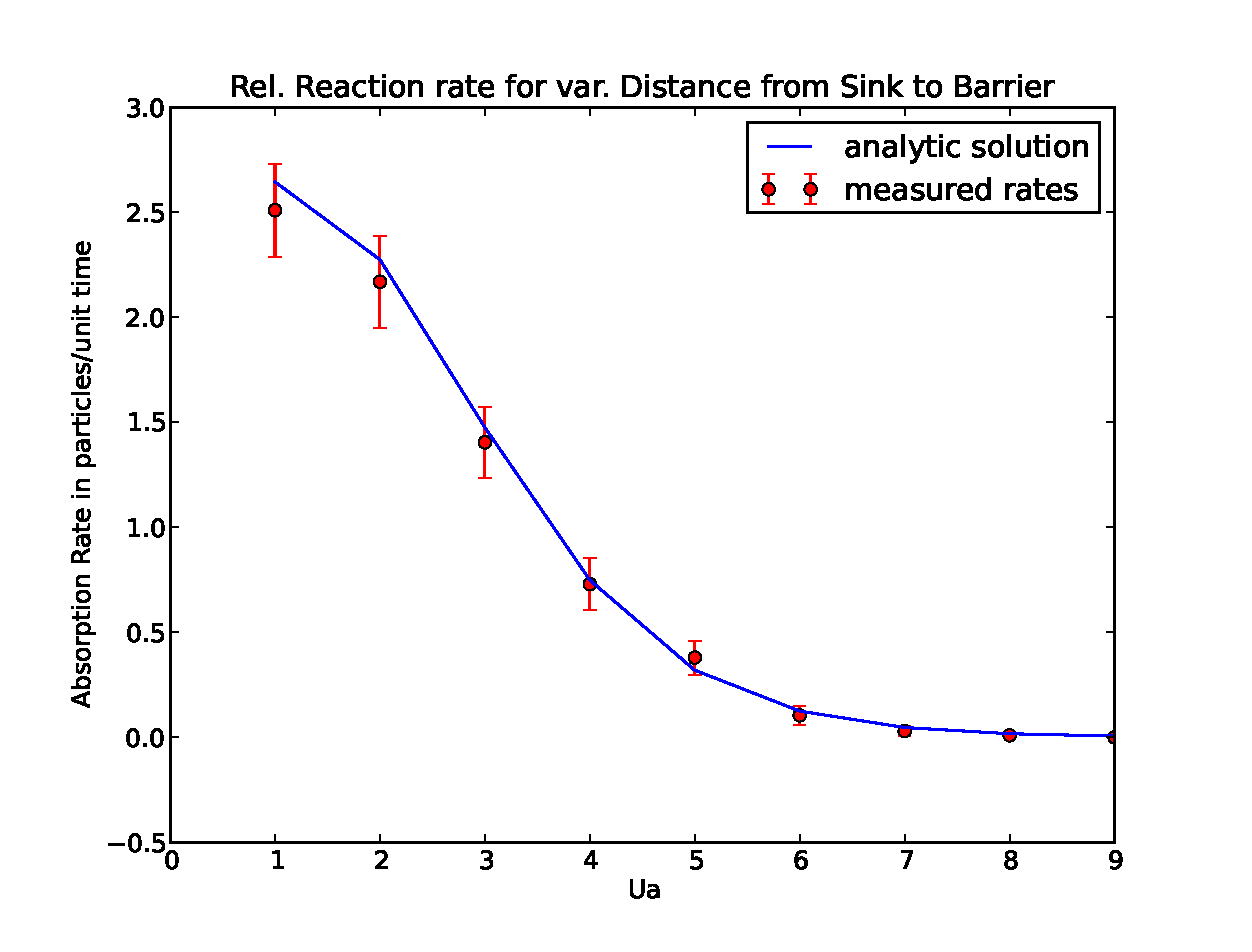
\includegraphics[width=.95 \textwidth, keepaspectratio]{plots/cp/uo/Kabs.eps}
\end{minipage}\begin{minipage}{.5 \textwidth}
    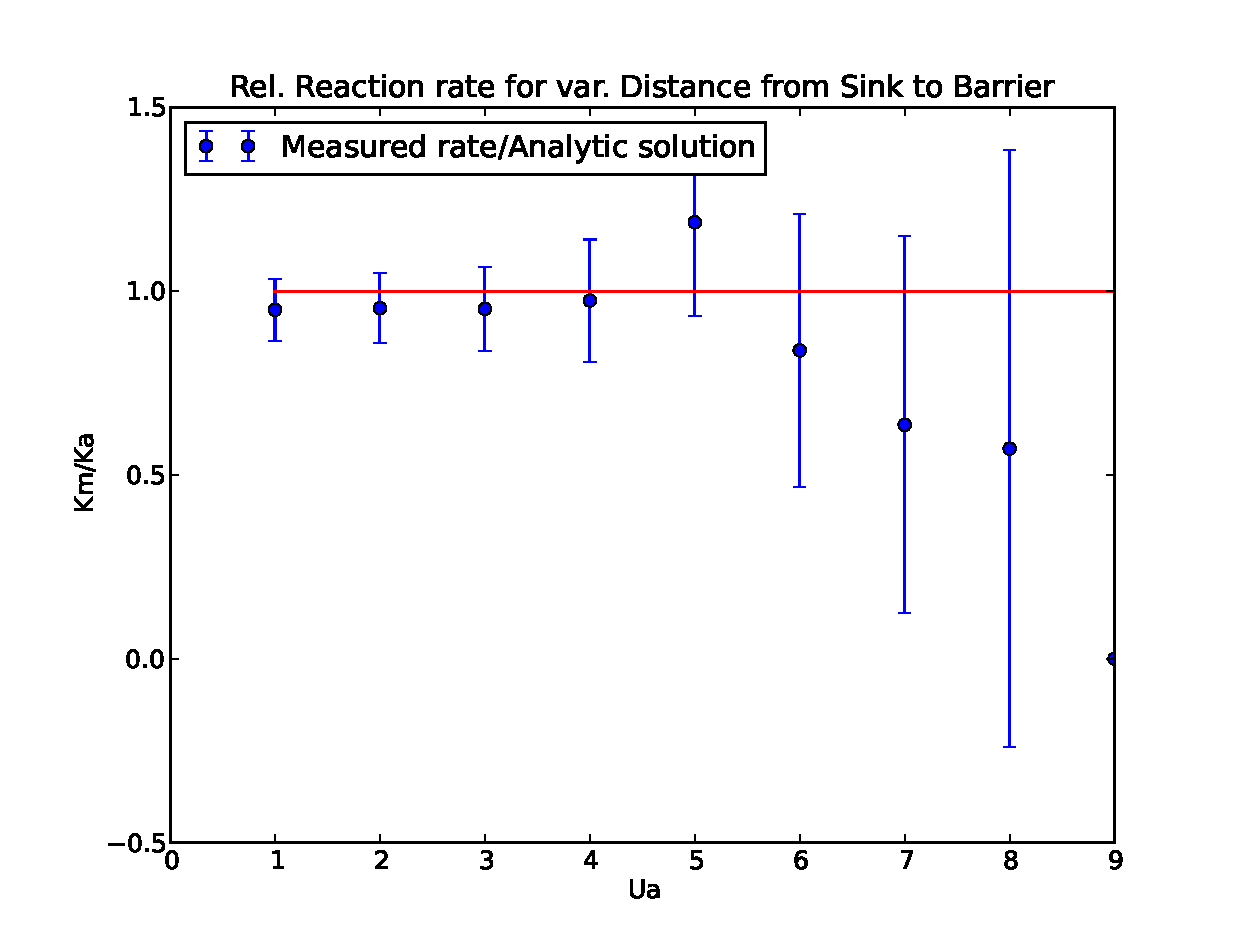
\includegraphics[width=.95 \textwidth, keepaspectratio]{plots/cp/uo/Krel.eps}
\end{minipage}
\caption{Absolute and relative Absorption rate for varying $U_0$}
\label{fig:KU0Cp}
\end{figure}


%\subsubsection{Varying Barrier Steepness ($U_n$)}
%\begin{figure}[H]
%\centering
%\begin{minipage}{.5 \textwidth}
%    \centering
%    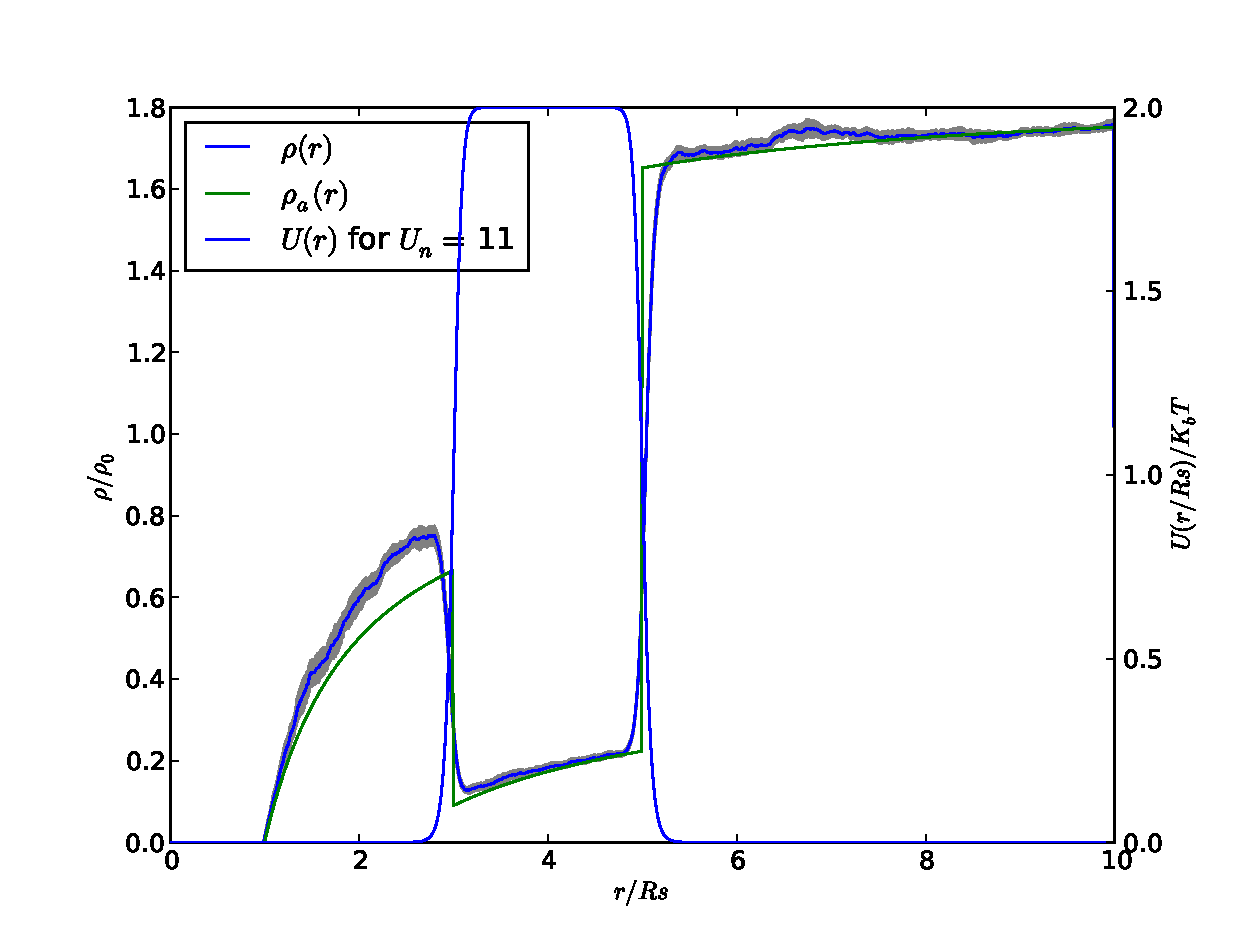
\includegraphics[width=.95 \textwidth, keepaspectratio]{plots/cp/un/Un11.eps}
%\end{minipage}\begin{minipage}{.5 \textwidth}
%    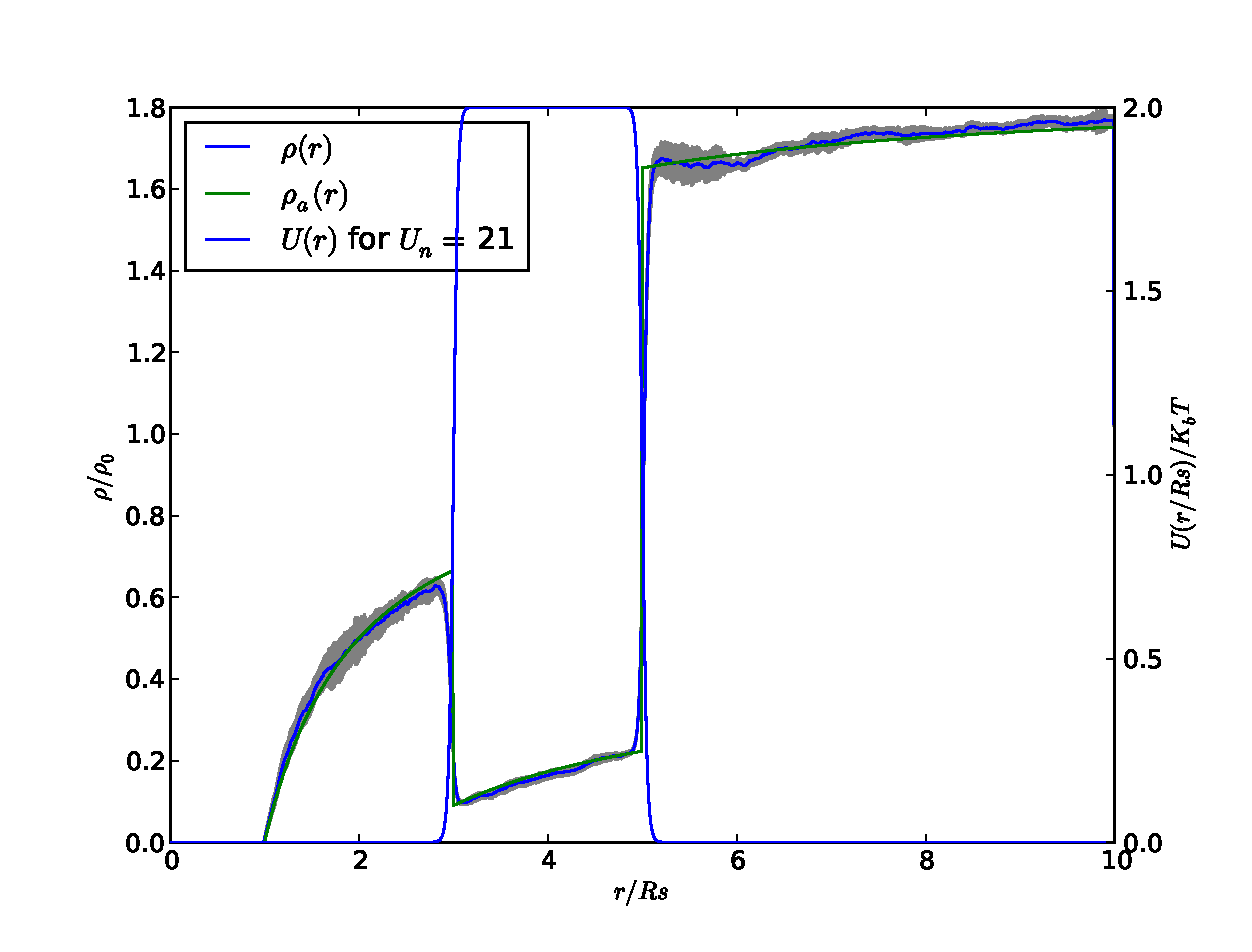
\includegraphics[width=.95 \textwidth, keepaspectratio]{plots/cp/un/Un21.eps}
%\end{minipage}
%\begin{minipage}{.5 \textwidth}
%    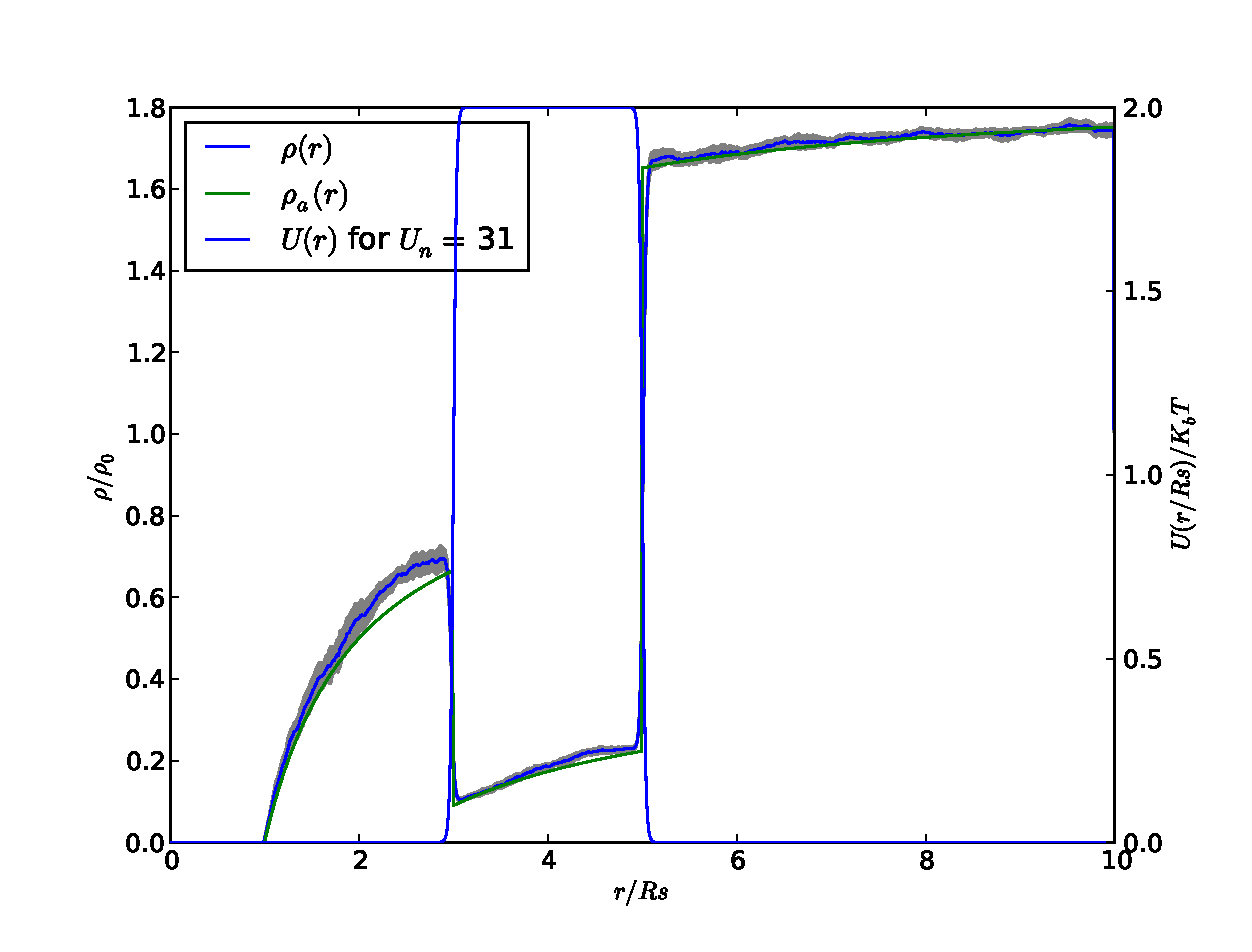
\includegraphics[width=.95 \textwidth, keepaspectratio]{plots/cp/un/Un31.eps}
%\end{minipage}\begin{minipage}{.5 \textwidth}
%    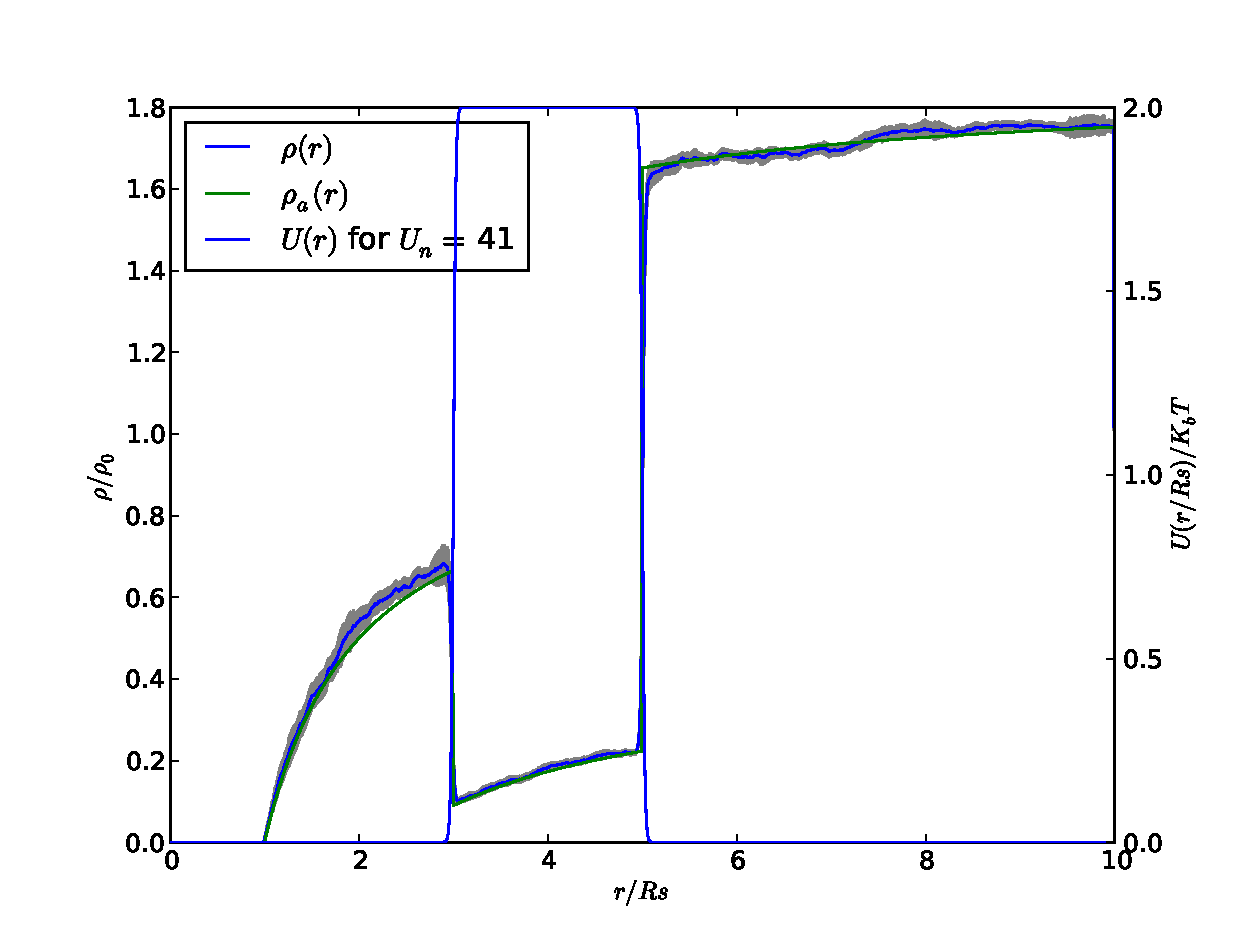
\includegraphics[width=.95 \textwidth, keepaspectratio]{plots/cp/un/Un41.eps}
%\end{minipage}
% 
%    \caption{Density Profile for varying $U_n$}
%    \label{fig:RhoUnCp}
%\end{figure}

The simulation results obviously fit the analytic solution. Same holds for the calculated reaction rates as presented in the following Plot:
\begin{figure}[H]
\centering
\begin{minipage}{.5 \textwidth}
    \centering
    \includegraphics[width=.95 \textwidth, keepaspectratio]{plots/cp/un/Kabs.eps}
\end{minipage}\begin{minipage}{.5 \textwidth}
    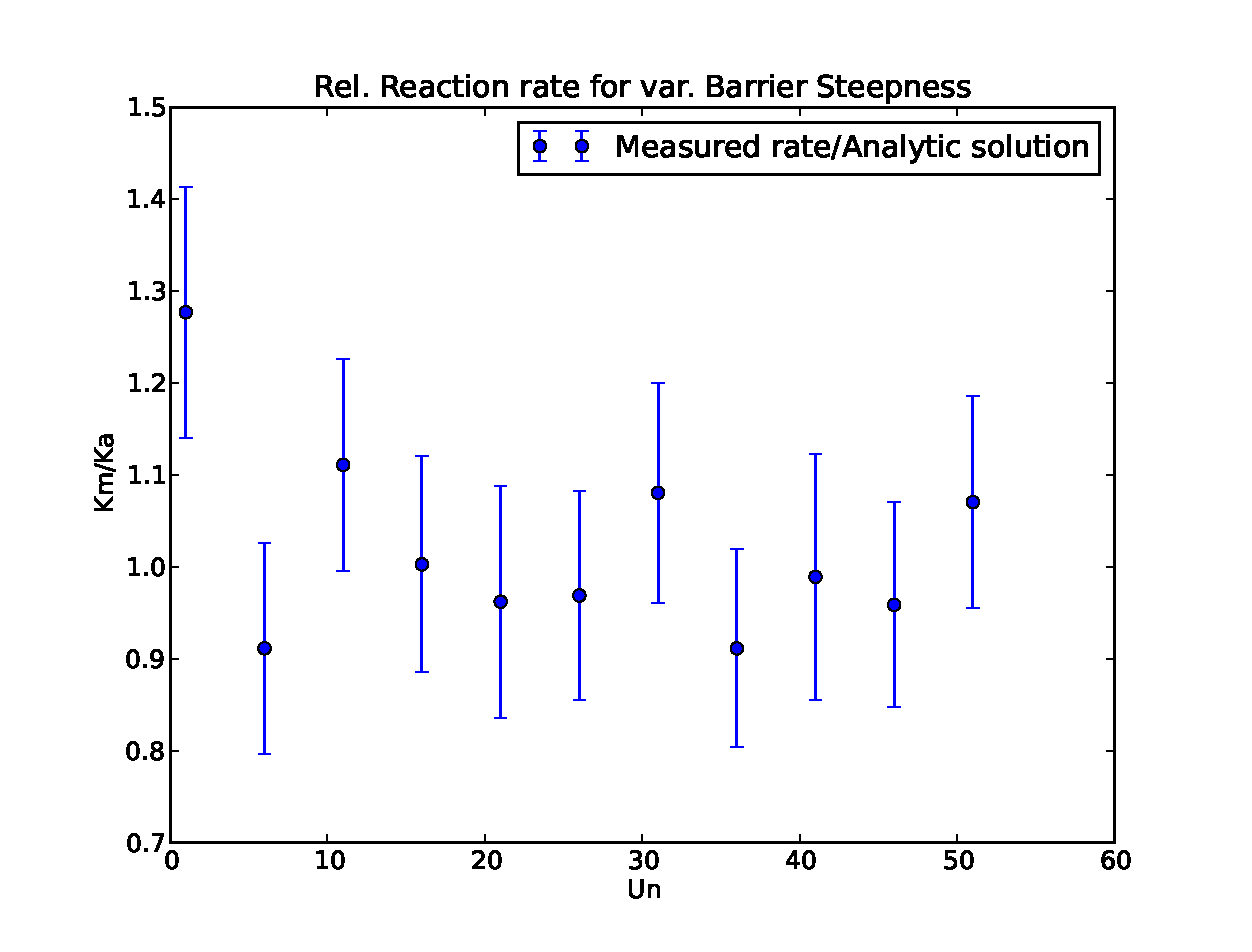
\includegraphics[width=.95 \textwidth, keepaspectratio]{plots/cp/un/Krel.eps}
\end{minipage}
\caption{Absolute and relative Absorption rate for varying $U_n$}
\label{fig:KUnCP}
\end{figure}


%\subsubsection{Varying Barrier Width}
%\begin{figure}[H]
%\centering
%\begin{minipage}{.5 \textwidth}
%    \centering
%    \includegraphics[width=.95 \textwidth, keepaspectratio]{plots/cp/ub/Ua1.eps}
%\end{minipage}\begin{minipage}{.5 \textwidth}
%    \includegraphics[width=.95 \textwidth, keepaspectratio]{plots/cp/ub/Ua3.eps}
%\end{minipage}
%\begin{minipage}{.5 \textwidth}
%    \includegraphics[width=.95 \textwidth, keepaspectratio]{plots/cp/ub/Ua5.eps}
%\end{minipage}\begin{minipage}{.5 \textwidth}
%    \includegraphics[width=.95 \textwidth, keepaspectratio]{plots/cp/ub/Ua5.eps}
%\end{minipage}
% 
%    \caption{Density Profile for varying $U_b$}
%    \label{fig:RhoUbCp}
%\end{figure}
%
%The simulation results obviously fit the analytic solution. Same holds for the calculated reaction rates as presented in the following Plot:
%\begin{figure}[H]
%\centering
%\begin{minipage}{.5 \textwidth}
%    \centering
%    \includegraphics[width=.95 \textwidth, keepaspectratio]{plots/cp/ub/Kabs.eps}
%\end{minipage}\begin{minipage}{.5 \textwidth}
%    \includegraphics[width=.95 \textwidth, keepaspectratio]{plots/cp/ub/Krel.eps}
%\end{minipage}
%\caption{Absolute and relative Absorption rate for varying $U_b$}
%\label{fig:KUbCp}
%\end{figure}


